% !TeX spellcheck = en_GB
% !TeX program = pdflatex
%
% LetzCV-sleek 1.0 LaTeX template
% Author: Andreï V. Kostyrka, University of Luxembourg
%
% This template fills the gap in the available variety of templates
% by proposing something that is not a custom class, not using any
% hard-coded settings deeply hidden in style files, and provides
% a handful of custom command definitions that are as transparent as it gets.
% Developed at the University of Luxembourg.
%
% *NOTHING IS HARCODED, and never should be.*
%
% Target audience: applicants in the IT industry, or business in general
%
% The main strength of this template is, it explicitly showcases how
% to break the flow of text to achieve the most flexible right alignment
% of dates for multiple configurations.

\documentclass[11pt, a4paper]{article}

\usepackage[T1]{fontenc}
\usepackage[utf8]{inputenc}
\usepackage[british]{babel}
\usepackage[left = 0mm, right = 0mm, top = 0mm, bottom = 0mm]{geometry}
\usepackage[stretch = 25, shrink = 25]{microtype}
\usepackage{graphicx}
\usepackage{xcolor}
\usepackage{marvosym}
\usepackage{eurosym}
\usepackage{fontawesome5}

\usepackage{enumitem}
\setlist{
    parsep = 0pt,
    topsep = 0pt,
    partopsep = 1pt,
    itemsep = 1pt,
    leftmargin = 6mm
}

\usepackage{FiraSans}
\renewcommand{\familydefault}{\sfdefault}

\definecolor{cvblue}{HTML}{304263}

%%%%%%% USER COMMAND DEFINITIONS %%%%%%%%%%%%%%%%%%%%%%%%%%%
% These are the real workhorses of this template
\newcommand{\dates}[1]{\hfill\mbox{\textbf{#1}}} % Bold stuff that doesn’t got broken into lines
\newcommand{\is}{\par\vskip.5ex plus .4ex} % Item spacing
\newcommand{\smaller}[1]{{\small\ #1}}
\newcommand{\headleft}[1]{
    \vspace*{3ex}\textsc{\textbf{#1}}\par%
    \vspace*{-1.5ex}\hrulefill\par\vspace*{0.7ex}
}
\newcommand{\headright}[1]{
    \vspace*{1.5ex}\textsc{\Large\color{cvblue}#1}\par%
    \vspace*{-2ex}{\color{cvblue}\hrulefill}\par
}
%%%%%%%%%%%%%%%%%%%%%%%%%%%%%%%%%%%%%%%%%%%%%%%%%%%%%%%%%%%%

\usepackage[colorlinks = true, urlcolor = white, linkcolor = white]{hyperref}
\usepackage{mycounters} % local

\begin{document}

% Style definitions -- killing the unnecessary space and adding the skips explicitly
\setlength{\topskip}{0pt}
\setlength{\parindent}{0pt}
\setlength{\parskip}{0pt}
\setlength{\fboxsep}{0pt}
\pagestyle{empty}
\raggedbottom

\begin{minipage}[t]{0.33\textwidth} %% Left column -- outer definition
    \colorbox{cvblue!90}{
        \color{white} %% LEFT BOX
        \kern0.09\textwidth\relax% Left margin provided explicitly
        \begin{minipage}[t][297mm][t]{0.82\textwidth}
            \raggedright
            \vspace*{2.5ex}

            \Large Dr.~Tom \textbf{\textsc{de Geus}} \normalsize

            % Centering without extra vertical spacing
            \null\hfill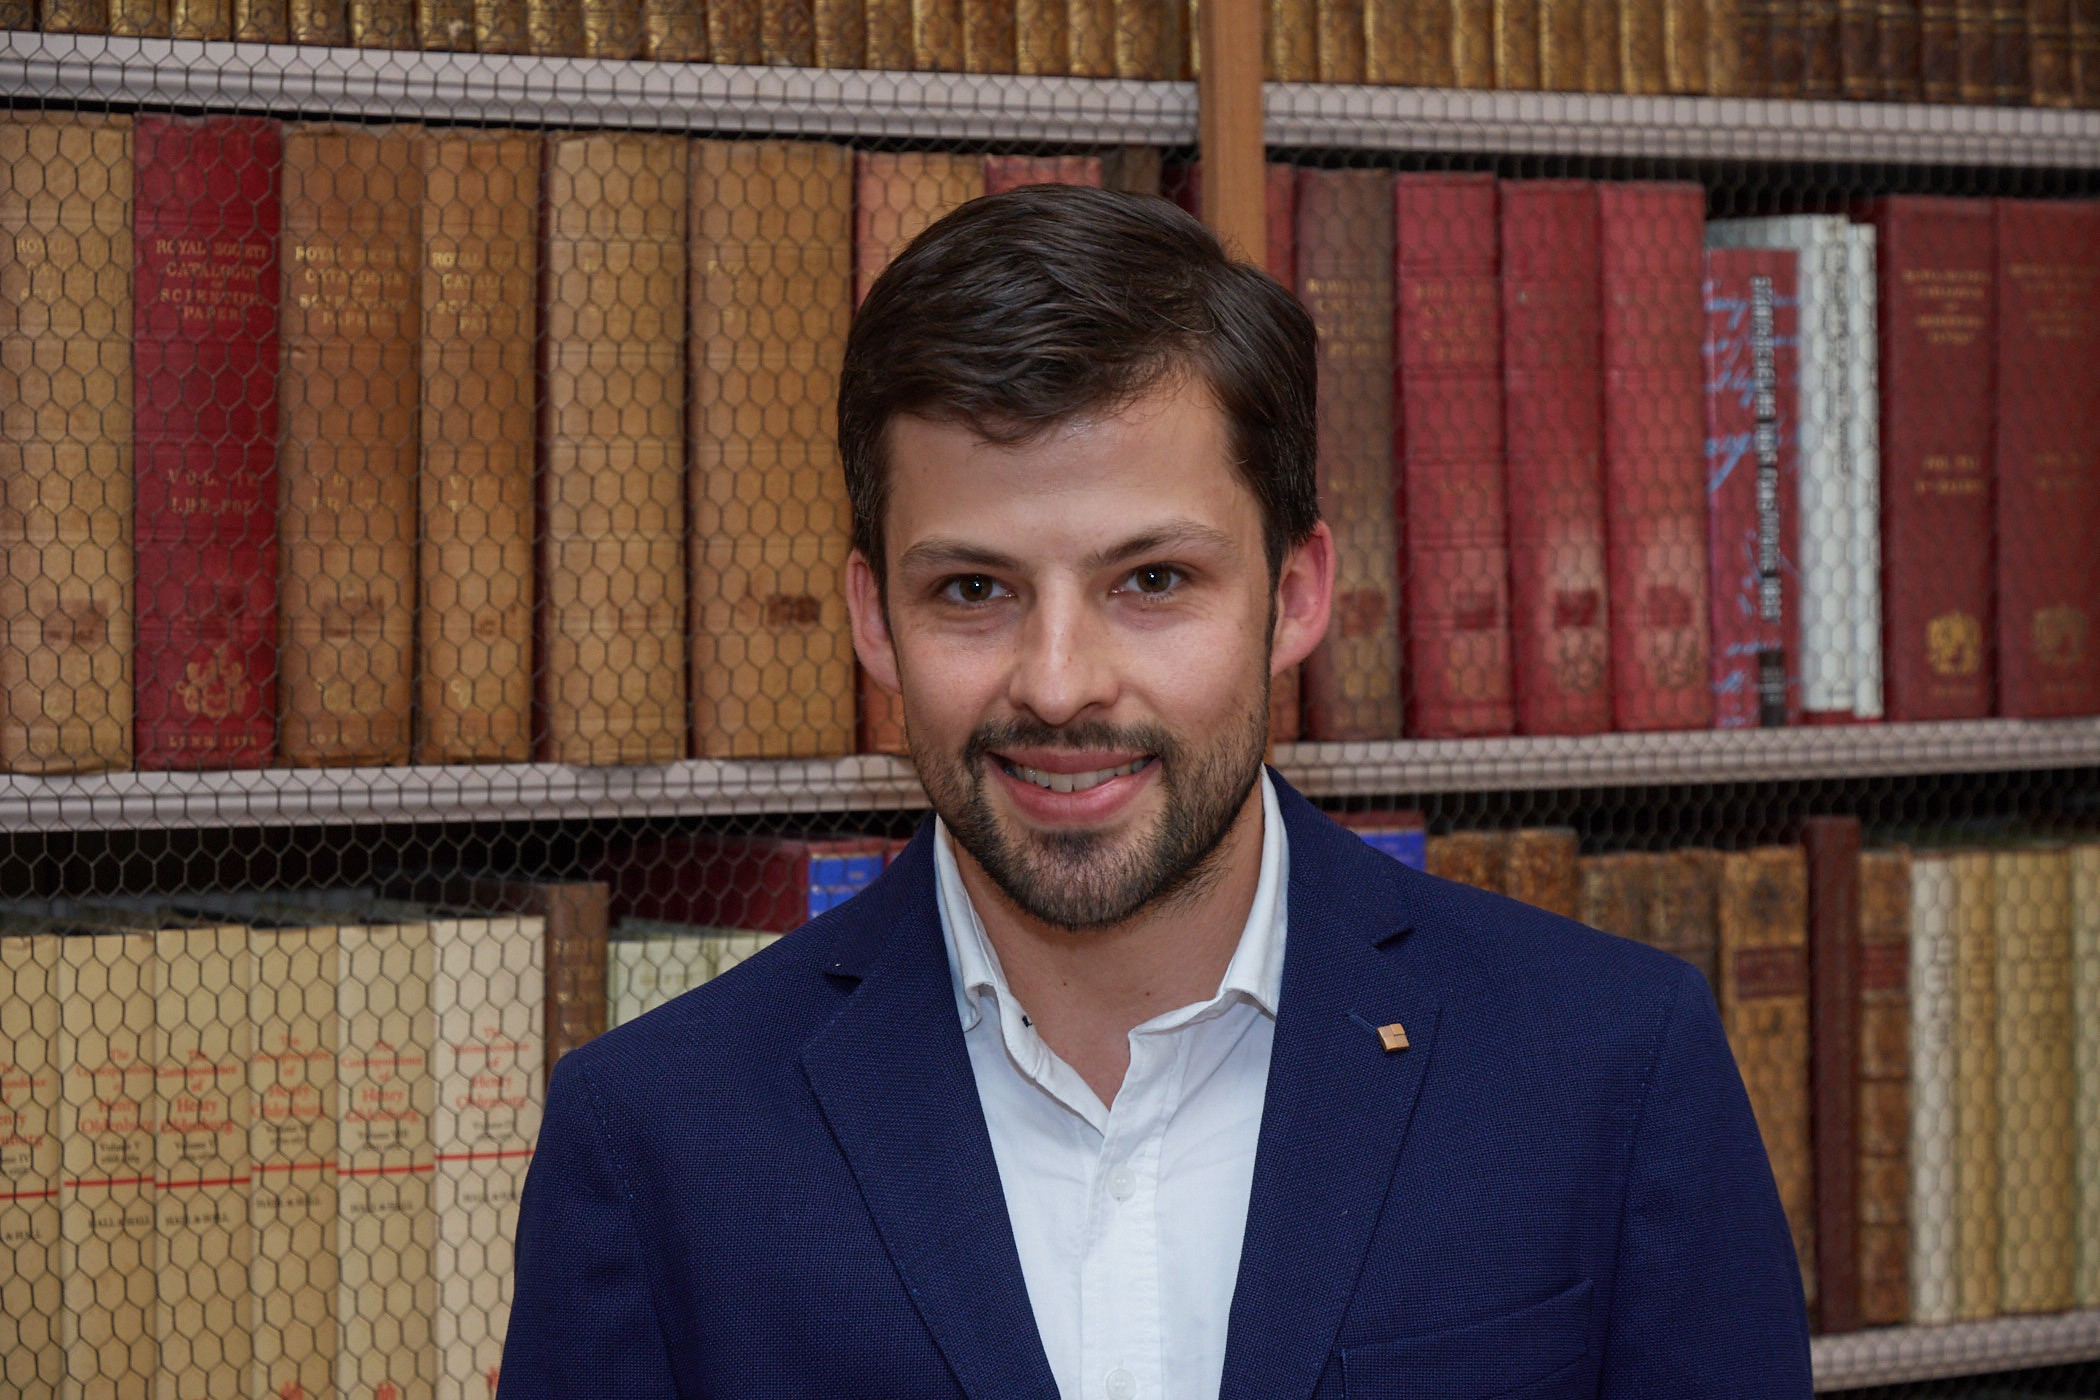
\includegraphics[width=0.9\textwidth]{tom.jpg}\hfill\null

            \vspace*{0.5ex}

            \headleft{Profile}
            Scientific leader with extensive experience connecting engineering, physics, materials science and applied research.
            Experienced in leading interdisciplinary collaborations, managing research projects and funding,
            developing talent, and translating complex scientific challenges into effective shared solutions.
            Passionate about building research infrastructures that enable outstanding science through excellent service, training and collaboration.
            
            \headleft{Assets}
            \begin{itemize}
                \item CHF 737k competitive research funding managed.
                \item 15+ years interdisciplinary research.
                \item IP expertise.
                \item Extensive teaching \& \\ 30+ student supervisions.
                \item Scientific communication in four languages.
            \end{itemize}

            \headleft{Contact details}
            \small
            \MVAt \hspace{0.5em} {\small \MySourceMail} \\
            [0.8ex]
            \Telefon \hspace{0.5em} +41\,77\,993\,72\,35 \\
            [0.8ex]
            \Mundus \hspace{0.5em} \MySourceSite \\
            [0.8ex]
            % \Letter\ Chemin du Parc-de-Valency 11 \\
            \Letter~\hspace{0.5em}
            \begin{minipage}[c]{\textwidth}
                Chemin du Parc-de-Valency 11 \\
                CH-1004 Lausanne
            \end{minipage}
            \\
            [0.8ex]
            \MySourceGitHub{\faIcon{github}} | \MySourceStackOverflow{\faIcon{stack-overflow}} | \MySourceLinkedIn{\faIcon{linkedin}} | \MySourceGoogleScholar{\faIcon{graduation-cap}} | \MySourceORCID{\faIcon{orcid}}
            \normalsize

            \headleft{Personal information}
            Year of birth: \textbf{1985} \\
            [0.5ex] Citizenship: \textbf{The Netherlands} \\
            [0.5ex] Residency: \textbf{Switzerland} {\tiny (C-permit)} \\
            [0.5ex] Civil status: \textbf{Married} \\
            [0.5ex] Languages: \\
            [0.5ex]
            \textbf{English} (C2), \textbf{French} (C2), \textbf{German} (C2/C1), \textbf{Dutch} (native)

        \end{minipage}%
        \kern0.09\textwidth\relax%%Right margin provided explicitly to stretch the colourbox
    }
\end{minipage}% Right column
\hskip2.5em% Left margin for the white area
\begin{minipage}[t]{0.56\textwidth}
    \hypersetup{urlcolor = cvblue, linkcolor = cvblue}

    \setlength{\parskip}{0.8ex}% Adds spaces between paragraphs; use \\ to add new lines without this space. Shrink this amount to fit more data vertically

    \vspace{2ex}

    \headright{Experience}

    \begin{itemize}
        \item
        \textbf{\textsc{Patent expert \& examiner}} \dates{\MyDateIPI}
        \vspace*{0.1eM}
        \\
        \textit{Swiss Federal Institute of Intellectual Property (Switzerland)}
        \vspace*{0.2eM}
        \smaller{%
            \begin{itemize}
                \item Managed a large portfolio of technically diverse patent dossiers under strict legal deadlines.
                \item Communicating with inventors and patent attorneys.
                \item Analysing technologies across many disciplines.
                \item Understanding innovation ecosystem.
                \item Prioritisation under deadlines.
                \item Member of communication task force.
            \end{itemize}
        }
        \vspace*{0.2eM}
        \item
        \textbf{\textsc{Senior researcher Physics}} \dates{\MyDateAmbizione}
        \vspace*{0.1eM}
        \\
        \textit{EPFL (Switzerland) -- Funding: FNSF Ambizione (Switzerland)}
        \vspace*{0.2eM}
        \smaller{%
            \begin{itemize}
                \item Acquired and managed CHF 567k SNSF Ambizione project.
                \item Established and coordinated interdisciplinary collaborations.
                \item Supervised bachelor, master and PhD researchers.
                \item Managed project planning, budgets and deliverables.
                \item Conducted internationally recognised research.
                \item Subjects: tribology, fracture, earthquakes, glasses, complex systems.
                \item Proposal of a novel, interdisciplinary, theory of friction.
                \item Delivery of top journal publications and conference presentations.
                \item Design, implementation, execution high-performance computations.
                \item Reviews for top journals.
                \item Data-champion.
            \end{itemize}
        }
        \vspace*{0.2eM}
        \item
        \textbf{\textsc{Postdoctoral researcher Physics}} \dates{\MyDateRubicon}
        \vspace*{0.1eM}
        \\
        \textit{EPFL (Switzerland) -- Funding: NWO Rubicon (The Netherlands)}
        \vspace*{0.2eM}
        \smaller{%
            \begin{itemize}
                \item Acquisition and management of funding (160 k\euro).
                \item Delivery of top journal publications and conference presentations.
                \item Co-supervision bachelor students.
                \item Teaching assistant statistical physics (physics).
                \item Teaching assistant continuum mechanics (civil engineering).
                %\item Design, implementation, execution high-performance computations.
                %\item Reviews for top journals.
            \end{itemize}
        }
        \vspace*{0.2eM}
        \item
        \textbf{\textsc{Postdoctoral researcher Valorization}} \dates{\MyDateValorization}
        \vspace*{0.1eM}
        \\
        \textit{M2i \& Tata Steel (The Netherlands)}
        \vspace*{0.2eM}
        \smaller{%
            \begin{itemize}
                \item Acquisition and management of funding (10 k\euro).
                \item Developed industrial tool for scanning electron microscopy.
            \end{itemize}
        }
        \vspace*{0.2eM}
        \item
        \textbf{\textsc{Research internship}} \dates{\MyDateHarvard}
        \vspace*{0.1eM}
        \\
        \textit{Harvard University (United States)}
        \vspace*{0.2eM}
        \smaller{%
            \begin{itemize}
                \item Design and analysis of a 3D meta-material.
                \item Development of numerical tools.
            \end{itemize}
        }
    \end{itemize}

    \vspace*{-0.5eM}
    \headright{Education}

    \begin{itemize}
        \item
        \textbf{\textsc{PhD Mechanical Engineering (cum laude)}} \dates{\MyDatePhD}
        \vspace*{0.1eM}
        \\
        \textit{Eindhoven University of Technology (The Netherlands)}
        \vspace*{0.2eM}
        \smaller{%
            \begin{itemize}
                \item Part of, experimental-theoretical, Public-Private-Partnership \\
                (Eindhoven University, Material Innovation Institute M2i, Tata Steel).
                \item Experimental-theoretical research on fracture of advanced steels\\
                in close collaboration with electron microscopy specialists.
                \item Topic: mechanics \& fracture of high-grade steel.
                \item \href{https://www.geus.me/education.html\#doctor-of-philosophy}{
                    Martinus van Marum award (12.5 k\euro) for:
                    Best PhD thesis\\in five years in the engineering sciences%
                }, and various other awards.
                %\item Various awards.
                \item Delivery of journal publications and conference presentations.
                \item Co-supervision of bachelor and master students.
                \item Teaching finite element method, programming, and design-based learning.
            \end{itemize}
        }
        \vspace*{0.2eM}
        \item
        \textbf{\textsc{MSc/BSc Mechanical Eng.~(great appreciation)}} \dates{\MyDateBScMSc}
        \vspace*{0.1eM}
        \\
        \textit{Eindhoven University of Technology (The Netherlands)}
        \vspace*{0.2eM}
        \smaller{%
            \begin{itemize}
                \item Specialization: mechanics of materials.
                \item Elective courses mathematics (numerical solvers).
                \item Minor: entrepreneurship.
                \item Winner entrepreneurship award (1 k\euro).
            \end{itemize}
        }
        \vspace*{0.2eM}
    \end{itemize}

\end{minipage}

\begin{minipage}[t]{0.1\textwidth} %% Left column -- outer definition
\end{minipage}% Right column
\hskip2.5em% Left margin for the white area
\begin{minipage}[t]{0.9\textwidth}
    \hypersetup{urlcolor = cvblue, linkcolor = cvblue}

    \setlength{\parskip}{0.8ex}% Adds spaces between paragraphs; use \\ to add new lines without this space. Shrink this amount to fit more data vertically

    \vspace{2ex}

    \headright{Professional strenghts}

    \begin{itemize}
        \item \textbf{\textsc{Analytical thinking}}:
        \begin{itemize}
            \item Combining theoretical physics \& mechanics.
            \item Designing and performing high-performance computing based on collaborative open-source tools.
        \end{itemize}
        \item \textbf{\textsc{Critical thinking}}:
        \begin{itemize}
            \item \MySourceStickSlip{Proposing a novel theory of friction} (despite it being an old and vast subject).
            \item Performing patent assessments (and considering solutions in case of problems).
        \end{itemize}
        \item \textbf{\textsc{Creativity}}:
        \begin{itemize}
            \item Combining knowledge from various disciplines.
            \item Proposing novel simple models by abstraction.
        \end{itemize}
        \item \textbf{\textsc{Adaptability}}:
        \begin{itemize}
            \item Integrating in Switzerland.
            \item Developing proficiency in various scientific fields.
            \item Transitioning between various professions (academia and public federal administration).
            %\item (Student job) Advising on and operating of rental (heavy) construction-equipment.
        \end{itemize}
    \end{itemize}

    \headright{Project management experience}

    \begin{itemize}
        \item \textbf{\textsc{Uniting}}:
        \begin{itemize}
            \item Initiating and fostering various interdisciplinary collaborations.
        \end{itemize}
        \item \textbf{\textsc{Prioritising \& Accountability}}:
        \begin{itemize}
            \item Balancing ad-hoc and permanent solutions.
            \item Anticipating deadlines, co-workers and other third parties.
        \end{itemize}
        \item \textbf{\textsc{Achieving Results, Persistence \& Resilience}}:
        \begin{itemize}
            \item Accomplishing goals \MySourceGrants{Ambizione grant}.
            \item \MySourcePublications{Publishing in PNAS, Physical Review Letters, and other top journals\ (\MySourceGoogleScholar{\MyTextCitations})}.
            \item (Non-professional) \MySourceChampionSuisse{Becoming Swiss rowing champion}.
        \end{itemize}
        \item \textbf{\textsc{Budgeting}}:
        \begin{itemize}
            \item Managing research project budgets.
            \item (Volunteering) Managing sport club budget.
        \end{itemize}
    \end{itemize}

    \headright{Leadership experience}

    \begin{itemize}
        \item \textbf{\textsc{Inspiring}}:
        \begin{itemize}
            \item Proposing and directing challenging student projects.
            \item Finishing \MySourceTdL{world's longest rowing race on closed water}, twice.
            \item Performing open science \& \MySourceGitHub{open-source coding}.
        \end{itemize}
        \item \textbf{\textsc{Motivating, Guiding, Strategising, Decision-making}}:
        \begin{itemize}
            \item (Co)-Supervising \MySourceExcitations{a PhD} student, and \MySourceStudents{\mystudents~bachelor and master projects}.
            \item (Volunteering) Leading mountaineering \& rowing outings (both high-risk sports).
            \item (Student job) Being a high school tutor (mathematics and physics).
            \item Initiating a social awareness game at the beginning of the COVID-pandemic: \MySourceRTS{TV-interview RTS}.
        \end{itemize}
        \item \textbf{\textsc{Communicating}}:
        \begin{itemize}
            \item Recognised for creating collaborative, open and supportive research environments.
            \item Authoring scientific publications and giving conference presentations and seminars.
            \item Performing patent-assessments and novelty analyses.
            \item Providing an interview with the \MySourceHorizons{FNSF Horizons magazine}.
        \end{itemize}
        \item \textbf{\textsc{Delegating, Team development}}:
        \begin{itemize}
            \item Running various scientific collaborations.
            \item (Student job) Being a shift leader of a catering team in the football stadium of PSV.
            \item Taking a motivating role in a team (professionally and in sports).
        \end{itemize}
        \item \textbf{\textsc{Including}}:
        \begin{itemize}
            \item (Volunteering) Being a buddy of a student on the autistic spectrum.
            \item (Volunteering) Training of diverse rowers.
            \item (Volunteering) Training of field-hockey keepers.
        \end{itemize}
    \end{itemize}

\end{minipage}

\end{document}
